\section{Task 3}
\subsection{Development view}
\begin{figure}[H]
    \centering
    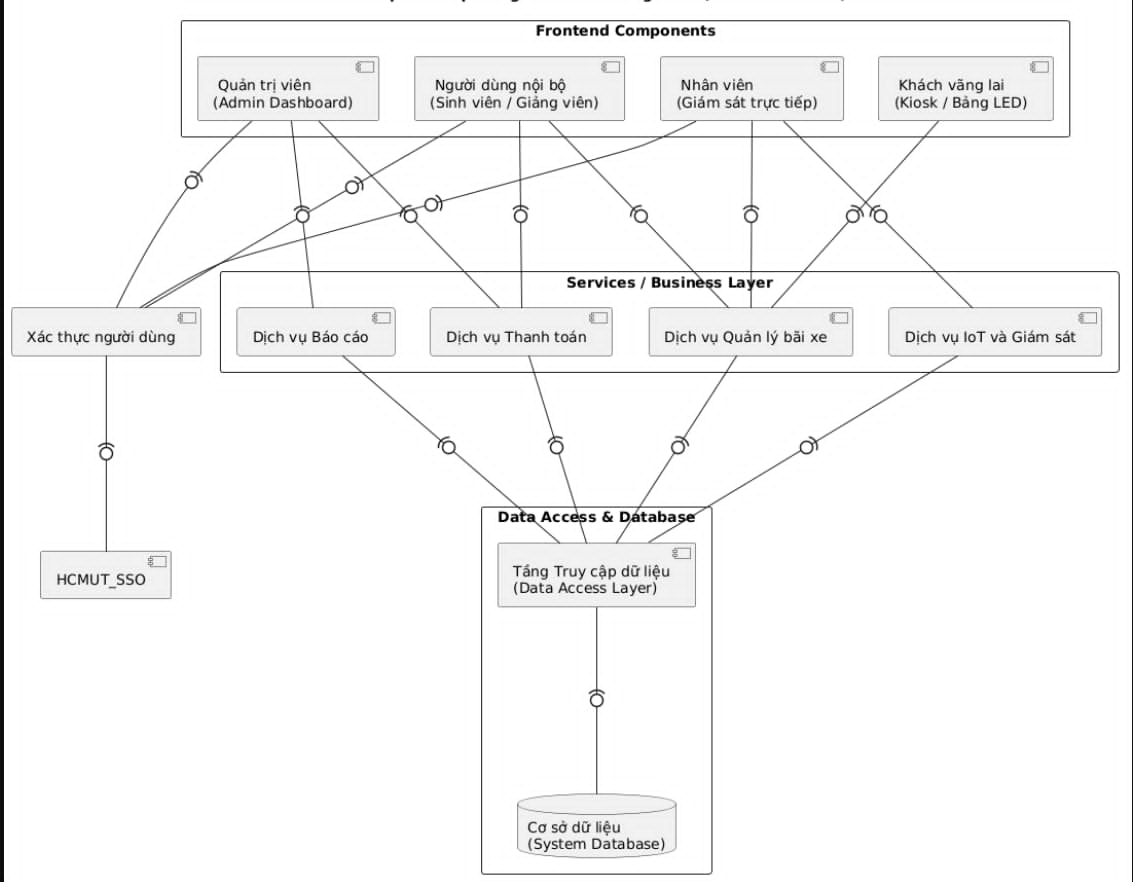
\includegraphics[width=1\linewidth]{Images/Task3/componentDiagram.jpg}
    \caption{Component Diagram cho toàn bộ hệ thống}
\end{figure}
\textbf{Mô tả:} Sơ đồ thành phần miêu tả cấu trúc của hệ thống, được chia thành ba tầng chính:Frontend, Services (Business Layer), Data Access và Database.
\begin{enumerate}
    \item \textbf{Front end components:} Tầng giao diện dành cho người dùng gồm 5 thành phần chính, ứng với các đối tượng sử dụng trong hệ thống.
    \begin{itemize}
        \item Quản trị viên (Admin Dashboard): quản trị toàn bộ hệ thống, dùng để theo dõi, giám sát toàn bộ hoạt động và đưa ra hành động yêu cầu sửa chữa khi cần.
        \item Người dùng nội bộ (Sinh viên/ Giảng viên): cho phép thành viên đăng nhập thông qua SSO. Đồng thời thực hiện các dịch vụ thanh toán cho các lượt giữ xe và hiển thị cho người dùng biết tình hình bãi xe.
        \item Nhân viên (Giám sát trực tiếp): nhân viên đăng nhập vào hệ thống thông qua SSO. Có vai trò quản lý tình hình bãi xe trực tiếp.
        \item Khách vãng lai (Kiosk/ Bảng LED): người dùng được cấp tạm 1 thẻ chứa thông tin tạm thời để sử dụng dịch vụ gửi xe.
    \end{itemize}
    \item \textbf{Services/ Business Layer:} Lớp dịch vụ xử lý toàn bộ logic  của hệ thống. Gồm các module chính:
    \begin{itemize}
        \item Dịch vụ báo cáo: báo cáo và phản hồi các sự cố xảy ra trong bãi giữ xe.
        \item Dịch vụ thanh toán: để giao dịch các khoản tiền phí giữ xe thông. Đối với người dùng nội bộ còn có thể liên kết với BkPay để giao dịch tiện lợi hơn.
        \item Dịch vụ Quản lý bãi xe: hiển thị số lượng chỗ trống còn lại để người sử dụng dịch vụ có thể biết và xác định chỗ đậu. Đồng thời giữ thông tin về chỗ đang đậu của người dùng giúp tìm kiếm xe dễ dàng hơn khi lấy.
        \item Dịch vụ IoT và Giám sát: bao gồm các cảm biến, thông báo chung để hiển thị cho người dùng cũng như nhân viên biết tình hĩnh bãi xe.
    \end{itemize}
    \item \textbf{Data Access \& Database:}
    \begin{itemize}
        \item Tầng truy cập dữ liệu (Data Access Layer): gửi yêu cầu truy xuất dữ liệu tới cơ sở dữ liệu.
        \item Cơ sở dữ liệu (System Database): Nhận yêu cầu và tìm kiếm dữ liệu được lưu trữ và trả về nếu có.
    \end{itemize}
\end{enumerate}
\newpage
\subsection{Deployment view}
\begin{figure}[H]
	\centering
	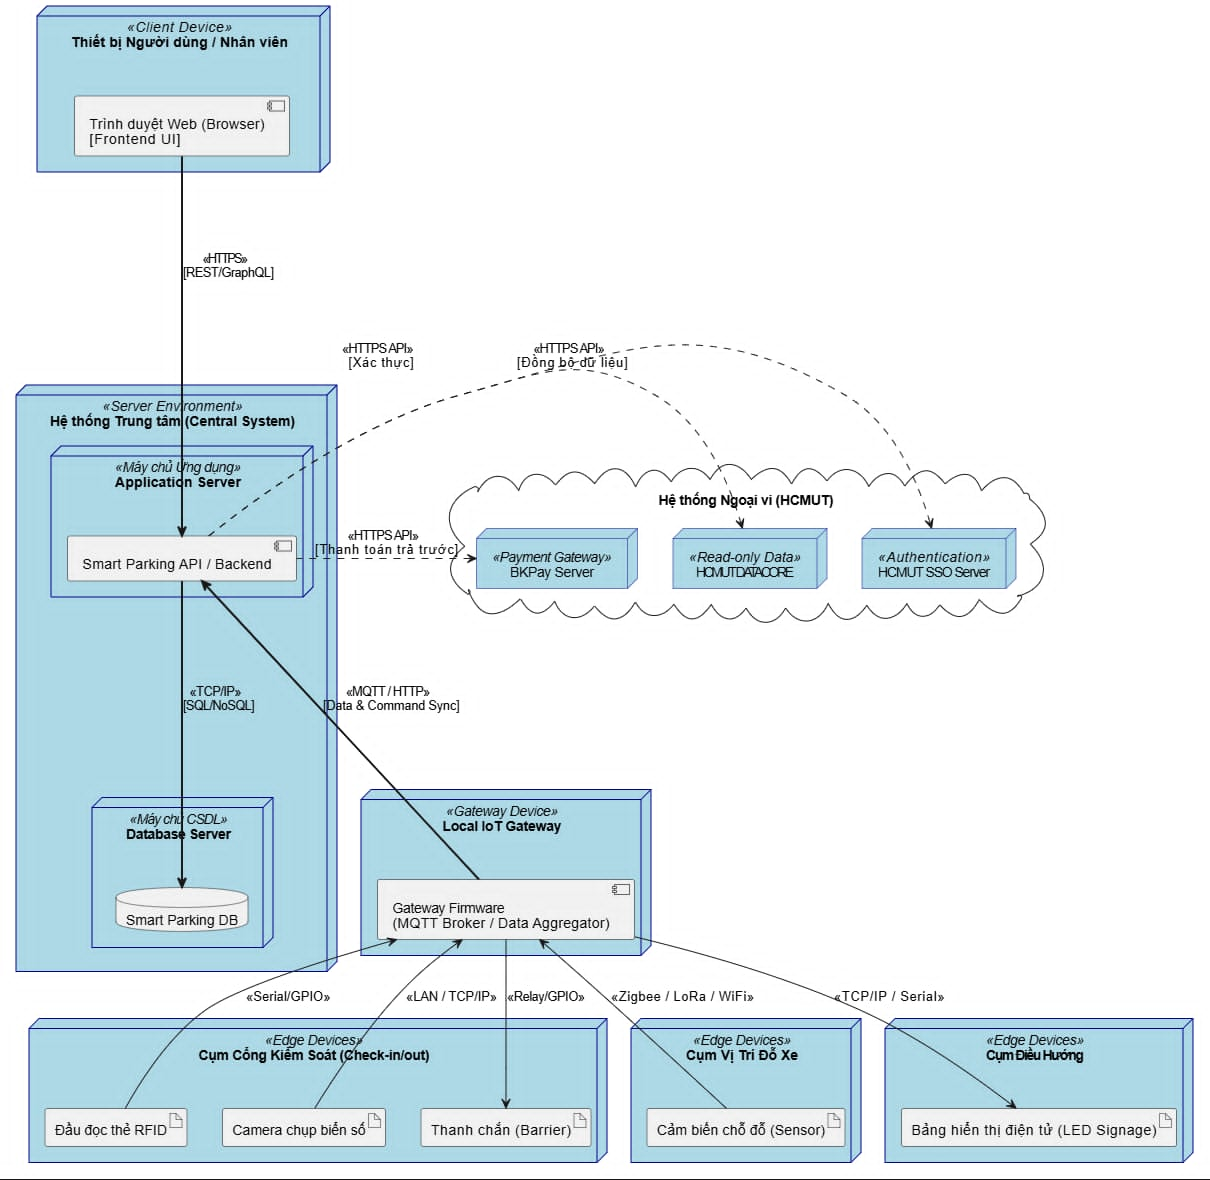
\includegraphics[width=1\linewidth]{Images/Task3/deployview.jpg}
	\caption{Deployment Diagram — Kiến trúc triển khai hệ thống}
\end{figure}
\newpage
\subsection{\textbf{Class Diagram and Method Script}}

\subsubsection{\textbf{Overview of Class Diagram}}

\subsubsection{\textbf{User Classes}}

\subsubsection{\textbf{Entity Classes}}

\subsubsection{\textbf{Service Classes}}

\noindent\textbf{AuthService}
\begin{itemize}
    \item \texttt{loginWithSSO(token: String): User}: Xử lý đăng nhập người dùng nội bộ thông qua \mbox{HCMUT\_SSO}. Phương thức nhận \texttt{token} từ giao diện hoặc luồng xác thực SSO, gửi token đến \texttt{SSOService} để kiểm tra, sau đó lấy thông tin người dùng và đối chiếu vai trò với DataCore khi cần. Kết quả trả về là đối tượng \texttt{User} nếu xác thực thành công; nếu token không hợp lệ, hệ thống không tạo phiên đăng nhập hợp lệ.
    \item \texttt{validateUser(user: User): boolean}: Kiểm tra đối tượng \texttt{User} trước khi cho phép truy cập hệ thống hoặc thực hiện chức năng cần phân quyền. Nội dung kiểm tra gồm mã định danh, email, vai trò, trạng thái tài khoản và quyền truy cập theo vai trò. Phương thức trả về \texttt{true} nếu người dùng hợp lệ, ngược lại trả về \texttt{false}.
\end{itemize}

\noindent\textbf{ParkingService}
\begin{itemize}
    \item \texttt{createSession(cardId: String): ParkingSession}: Tạo phiên gửi xe mới khi người dùng nội bộ hoặc khách vãng lai sử dụng thẻ tại cổng vào. Phương thức kiểm tra \texttt{cardId}, xác định loại thẻ, chọn chỗ đỗ phù hợp, ghi nhận thời gian vào bãi và khởi tạo \texttt{ParkingSession} ở trạng thái đang hoạt động. Kết quả trả về là phiên gửi xe mới nếu thẻ và chỗ đỗ hợp lệ.
    \item \texttt{closeSession(cardId: String): void}: Kết thúc phiên gửi xe khi người dùng quẹt thẻ tại cổng ra. Phương thức tìm phiên đang hoạt động theo \texttt{cardId}, ghi nhận thời gian ra, cập nhật trạng thái phiên, giải phóng chỗ đỗ và chuẩn bị dữ liệu cho bước tính phí hoặc thanh toán. Phương thức không trả về dữ liệu trực tiếp.
    \item \texttt{assignSpot(): ParkingSpot}: Chọn chỗ đỗ phù hợp cho phiên gửi xe mới dựa trên danh sách chỗ còn trống, trạng thái khu vực, vai trò người dùng và chính sách ưu tiên nếu có. Sau khi chọn được chỗ, hệ thống có thể đánh dấu chỗ là đang được sử dụng hoặc được giữ tạm thời. Kết quả trả về là \texttt{ParkingSpot} phù hợp.
    \item \texttt{updateStatus(): void}: Cập nhật trạng thái vận hành của bãi xe sau sự kiện xe vào, xe ra hoặc khi có dữ liệu mới từ IoT Gateway. Phương thức tổng hợp trạng thái phiên gửi xe, chỗ đỗ và khu vực để bảo đảm thông tin hiển thị gần thời gian thực. Phương thức không trả về dữ liệu trực tiếp.
\end{itemize}

\noindent\textbf{PaymentService}
\begin{itemize}
    \item \texttt{calculateFee(sessionId: String): double}: Tính phí gửi xe cho một phiên cụ thể. Phương thức tìm \texttt{ParkingSession} theo \texttt{sessionId}, tính thời lượng gửi xe, lấy chính sách giá hiện hành từ \texttt{PricingService}, sau đó tính số tiền cần thanh toán theo thời gian gửi, nhóm người dùng và ưu đãi nếu có. Kết quả trả về là số tiền dạng \texttt{double}.
    \item \texttt{processOnSitePayment(sessionId: String): boolean}: Xử lý thanh toán trực tiếp tại bãi xe, thường dùng cho khách vãng lai hoặc giao dịch tại cổng. Phương thức tính phí, tạo thông tin thanh toán, ghi nhận phương thức thanh toán và cập nhật trạng thái sau khi giao dịch được xác nhận. Kết quả trả về \texttt{true} khi thanh toán thành công, ngược lại trả về \texttt{false}.
    \item \texttt{processPrepaidPayment(sessionId: String): boolean}: Xử lý thanh toán bằng gói trả trước hoặc hình thức thanh toán định kỳ của người dùng nội bộ. Phương thức kiểm tra phiên gửi xe, xác định người dùng, kiểm tra gói trả trước hoặc chính sách đang áp dụng, sau đó ghi nhận giao dịch tương ứng. Kết quả trả về \texttt{true} nếu giao dịch hợp lệ và được ghi nhận.
\end{itemize}

\noindent\textbf{PricingService}
\begin{itemize}
    \item \texttt{getCurrentPolicy(role: Role): PricingPolicy}: Lấy chính sách giá hiện hành cho một nhóm người dùng. Phương thức sử dụng \texttt{role} để xác định đối tượng áp dụng như sinh viên, giảng viên, nhân viên, quản trị viên hoặc khách vãng lai. Kết quả trả về là \texttt{PricingPolicy} tương ứng.
    \item \texttt{updatePolicy(policy: PricingPolicy): void}: Cập nhật hoặc thay thế chính sách giá trong hệ thống. Chức năng này được dùng bởi quản trị viên khi thay đổi giá theo giờ, số phút miễn phí, phần trăm giảm giá hoặc nhóm người dùng được áp dụng. Phương thức nhận \texttt{policy} mới hoặc đã chỉnh sửa và không trả về dữ liệu trực tiếp.
\end{itemize}

\noindent\textbf{ReportService}
\begin{itemize}
    \item \texttt{generateReport(type: ReportType, dateRange: DateRange): Report}: Tạo báo cáo thống kê theo loại báo cáo và khoảng thời gian được chọn. Phương thức truy xuất dữ liệu về phiên gửi xe, giao dịch thanh toán, trạng thái khu vực hoặc tần suất sử dụng, sau đó tổng hợp thành nội dung báo cáo. Kết quả trả về là đối tượng \texttt{Report}.
    \item \texttt{exportReport(id: String, format: String): File}: Xuất báo cáo đã tạo thành tệp theo định dạng được yêu cầu. Phương thức tìm báo cáo theo \texttt{id}, kiểm tra \texttt{format}, tạo tệp và cung cấp kết quả cho người dùng tải xuống hoặc lưu trữ. Kết quả trả về là đối tượng \texttt{File}.
\end{itemize}

\noindent\textbf{IncidentService}
\begin{itemize}
    \item \texttt{reportIncident(desc: String, type: IncidentType): Incident}: Ghi nhận sự cố phát sinh trong quá trình vận hành bãi xe, bao gồm lỗi phần cứng, thiết bị IoT, cổng ra vào, thanh toán hoặc tình huống cần nhân viên xử lý. Phương thức tạo \texttt{Incident} với mô tả, loại sự cố, trạng thái ban đầu và người báo cáo nếu có. Kết quả trả về là sự cố mới được tạo.
    \item \texttt{resolveIncident(id: String): void}: Cập nhật trạng thái sự cố sau khi nhân viên hoặc quản trị viên xử lý xong. Phương thức tìm sự cố theo \texttt{id}, kiểm tra trạng thái hiện tại và chuyển sự cố sang trạng thái đã giải quyết khi thao tác hợp lệ. Phương thức không trả về dữ liệu trực tiếp.
    \item \texttt{notifyAdmin(incident: Incident): void}: Gửi thông báo đến quản trị viên khi có sự cố cần theo dõi hoặc xử lý. Nội dung thông báo có thể gồm loại sự cố, mô tả, thời điểm phát sinh và trạng thái hiện tại. Phương thức không trả về dữ liệu trực tiếp.
\end{itemize}

\noindent\textbf{ZoneService}
\begin{itemize}
    \item \texttt{getZoneStatus(): List<ParkingZone>}: Lấy danh sách trạng thái hiện tại của các khu vực trong bãi xe. Phương thức tổng hợp số chỗ trống, tổng số chỗ, trạng thái khu vực và dữ liệu cảm biến nếu có. Kết quả trả về là danh sách \texttt{ParkingZone}.
    \item \texttt{updateZoneStatus(zoneId: String): void}: Cập nhật trạng thái của một khu vực bãi xe cụ thể. Phương thức xác định số chỗ trống hiện tại trong khu vực, so sánh với tổng số chỗ và cập nhật trạng thái khu vực thành còn chỗ, gần đầy hoặc đầy. Phương thức không trả về dữ liệu trực tiếp.
    \item \texttt{suggestZone(role: Role): ParkingZone}: Đề xuất khu vực đỗ xe phù hợp dựa trên vai trò người dùng và trạng thái hiện tại của các khu vực. Hệ thống có thể ưu tiên khu vực dành cho nhóm người dùng tương ứng hoặc khu vực thay thế khi khu ưu tiên đã đầy. Kết quả trả về là \texttt{ParkingZone} được đề xuất.
\end{itemize}

\subsubsection{\textbf{Controller Classes}}

\noindent\textbf{AuthController}
\begin{itemize}
    \item \texttt{login(): void}: Tiếp nhận yêu cầu đăng nhập từ giao diện người dùng, lấy token hoặc dữ liệu xác thực cần thiết và gọi \texttt{AuthService.loginWithSSO()} để xử lý. Phương thức không có tham số trong class diagram và không trả về dữ liệu trực tiếp; kết quả được thể hiện qua phản hồi đăng nhập thành công hoặc thất bại.
    \item \texttt{logout(): void}: Tiếp nhận yêu cầu đăng xuất, hủy phiên đăng nhập hiện tại và xóa trạng thái phiên nếu cần. Phương thức không có tham số và không trả về dữ liệu trực tiếp.
\end{itemize}

\noindent\textbf{ParkingController}
\begin{itemize}
    \item \texttt{checkIn(): void}: Tiếp nhận yêu cầu vào bãi xe từ cổng vào sau khi người dùng quẹt thẻ hoặc thẻ vãng lai được cấp. Controller lấy dữ liệu thẻ từ request hoặc thiết bị đọc thẻ, gọi \texttt{ParkingService.createSession()} và điều phối mở barrier nếu phiên gửi xe được tạo thành công.
    \item \texttt{checkOut(): void}: Tiếp nhận yêu cầu ra khỏi bãi xe tại cổng ra. Controller lấy mã thẻ, gọi \texttt{ParkingService.closeSession()}, sau đó điều phối bước tính phí hoặc xác nhận thanh toán trước khi mở barrier. Phương thức không trả về dữ liệu trực tiếp.
    \item \texttt{getZoneStatus(): void}: Tiếp nhận yêu cầu xem trạng thái các khu vực bãi xe từ người dùng, nhân viên hoặc bảng hiển thị. Controller gọi \texttt{ZoneService.getZoneStatus()} và cung cấp dữ liệu trạng thái cho giao diện hoặc thiết bị hiển thị.
\end{itemize}

\noindent\textbf{PaymentController}
\begin{itemize}
    \item \texttt{payOnSite(): void}: Tiếp nhận yêu cầu thanh toán trực tiếp tại bãi xe. Controller lấy mã phiên gửi xe từ request hoặc từ thẻ, gọi \texttt{PaymentService.processOnSitePayment()} và trả kết quả thanh toán cho nhân viên hoặc thiết bị tại cổng.
    \item \texttt{payPrepaid(): void}: Tiếp nhận yêu cầu thanh toán bằng gói trả trước hoặc thanh toán định kỳ. Controller lấy thông tin phiên gửi xe hoặc người dùng, gọi \texttt{PaymentService.processPrepaidPayment()} và phản hồi kết quả xử lý cho giao diện.
\end{itemize}

\noindent\textbf{AdminController}
\begin{itemize}
    \item \texttt{configurePricing(): void}: Tiếp nhận yêu cầu cấu hình chính sách giá từ quản trị viên. Controller lấy thông tin chính sách mới từ giao diện, kiểm tra quyền thao tác cơ bản và gọi \texttt{PricingService.updatePolicy()} để cập nhật chính sách.
    \item \texttt{manageUsers(): void}: Tiếp nhận yêu cầu quản lý người dùng từ quản trị viên. Controller có thể gọi \texttt{DataCoreService.getUser()} hoặc \texttt{DataCoreService.syncUserList()} để lấy và đồng bộ dữ liệu người dùng từ \mbox{HCMUT\_DATACORE}, phục vụ kiểm tra thông tin và vai trò.
    \item \texttt{monitorSystem(): void}: Tiếp nhận yêu cầu giám sát trạng thái hệ thống từ quản trị viên. Controller tổng hợp trạng thái đồng bộ DataCore, kết nối IoT Gateway, trạng thái khu vực bãi xe và các sự cố đang tồn tại để hiển thị trên giao diện quản trị.
\end{itemize}

\noindent\textbf{ReportController}
\begin{itemize}
    \item \texttt{viewReport(): void}: Tiếp nhận yêu cầu xem báo cáo từ nhân viên hoặc quản trị viên. Controller lấy loại báo cáo, khoảng thời gian và tiêu chí lọc từ giao diện, sau đó gọi \texttt{ReportService.generateReport()} để tạo và hiển thị báo cáo.
    \item \texttt{exportReport(): void}: Tiếp nhận yêu cầu xuất báo cáo từ người dùng có quyền. Controller lấy mã báo cáo và định dạng tệp, gọi \texttt{ReportService.exportReport()} và cung cấp tệp báo cáo cho người dùng.
\end{itemize}

\noindent\textbf{IncidentController}
\begin{itemize}
    \item \texttt{submitIncident(): void}: Tiếp nhận yêu cầu ghi nhận sự cố từ nhân viên hoặc giao diện vận hành. Controller lấy mô tả và loại sự cố, gọi \texttt{IncidentService.reportIncident()} và phản hồi kết quả ghi nhận cho giao diện.
    \item \texttt{resolveIncident(): void}: Tiếp nhận yêu cầu xử lý hoặc đóng sự cố. Controller lấy mã sự cố, gọi \texttt{IncidentService.resolveIncident()} và cập nhật trạng thái sự cố trên giao diện nếu thao tác hợp lệ.
\end{itemize}

\subsubsection{\textbf{External System Classes}}

\noindent\textbf{SSOService}
\begin{itemize}
    \item \texttt{authenticate(token: String): User}: Đại diện cho thao tác xác thực người dùng thông qua \mbox{HCMUT\_SSO}. Hệ thống gửi \texttt{token} đến dịch vụ SSO để kiểm tra danh tính. Nếu token hợp lệ, dịch vụ trả về thông tin người dùng đã xác thực dưới dạng \texttt{User}.
\end{itemize}

\noindent\textbf{BKPayService}
\begin{itemize}
    \item \texttt{processPayment(amount: double): boolean}: Gửi yêu cầu thanh toán sang BKPay với số tiền cần xử lý. BKPay kiểm tra giao dịch, xử lý thanh toán và trả kết quả cho hệ thống Smart Parking. Phương thức trả về \texttt{true} nếu thanh toán thành công, ngược lại trả về \texttt{false}.
    \item \texttt{cancelPayment(txId: String): boolean}: Gửi yêu cầu hủy giao dịch thanh toán đã tạo trên BKPay. Phương thức được dùng khi giao dịch phát sinh lỗi, người dùng dừng thanh toán hoặc phiên gửi xe không còn hợp lệ. Kết quả trả về \texttt{true} nếu hủy thành công, ngược lại trả về \texttt{false}.
\end{itemize}

\noindent\textbf{DataCoreService}
\begin{itemize}
    \item \texttt{getUser(id: String): User}: Lấy thông tin người dùng từ \mbox{HCMUT\_DATACORE} theo mã định danh. Dữ liệu có thể gồm tên, email, vai trò và thông tin cần thiết để phân quyền trong hệ thống. Kết quả trả về là \texttt{User} nếu tìm thấy người dùng tương ứng.
    \item \texttt{syncUserList(): List<User>}: Đồng bộ danh sách người dùng từ \mbox{HCMUT\_DATACORE} về hệ thống Smart Parking. Phương thức hỗ trợ cập nhật danh sách người dùng và vai trò theo nguồn dữ liệu chính thức. Kết quả trả về là danh sách \texttt{User}.
    \item \texttt{checkSyncStatus(): SyncStatus}: Kiểm tra trạng thái đồng bộ giữa Smart Parking và \mbox{HCMUT\_DATACORE}. Kết quả được dùng để hiển thị trên màn hình quản trị hoặc phát hiện lỗi đồng bộ. Phương thức trả về \texttt{SyncStatus}.
\end{itemize}

\noindent\textbf{IoTGateway}
\begin{itemize}
    \item \texttt{sendCommand(command: String): void}: Gửi lệnh điều khiển từ hệ thống trung tâm đến IoT Gateway. Lệnh có thể liên quan đến cổng, bảng hiển thị, barrier hoặc thiết bị IoT khác trong bãi xe. Phương thức không trả về dữ liệu trực tiếp.
    \item \texttt{receiveData(): SensorData}: Nhận dữ liệu cảm biến từ IoT Gateway, bao gồm trạng thái chỗ đỗ, trạng thái thiết bị, thời điểm cập nhật và dữ liệu phục vụ giám sát gần thời gian thực. Kết quả trả về là \texttt{SensorData}.
    \item \texttt{openBarrier(): void}: Gửi yêu cầu mở barrier tại cổng ra hoặc cổng vào. Phương thức thường được gọi sau khi hệ thống xác nhận người dùng được phép vào bãi hoặc ra khỏi bãi. Phương thức không trả về dữ liệu trực tiếp.
    \item \texttt{getConnectionStatus(): boolean}: Kiểm tra trạng thái kết nối giữa hệ thống trung tâm và IoT Gateway. Phương thức trả về \texttt{true} nếu gateway hoạt động bình thường, ngược lại trả về \texttt{false}.
    \item \texttt{syncOfflineData(): void}: Đồng bộ dữ liệu được lưu tạm trong gateway khi kết nối với hệ thống trung tâm bị gián đoạn. Sau khi kết nối được khôi phục, gateway gửi lại dữ liệu chưa đồng bộ như trạng thái cảm biến, sự kiện vào ra hoặc bản ghi thiết bị. Phương thức không trả về dữ liệu trực tiếp.
\end{itemize}

\subsubsection{\textbf{Hardware/IoT Classes}}

\subsubsection{\textbf{Enumerations}}

